\BiChapter{基于视角增强的光场显著性目标检测}{TODO}
\label{chap:part4}
%
%
%
%
第三章从焦点感知的角度出发,设计了一种切片级探索多视角场景聚焦信息的显著性目标检测算法。
该方法注重对多视角三维场景的感知,以及不同视角对显著性预测的贡献程度,
实现了光场信息的深度挖掘以及多视角信息的高效探索。
%
%
本章从视角强化的角度出发,基于注意力机制引入视角增强模块,并通过前背景的补偿模块优化网络的训练,
实现了光场信息的充分挖掘。
%
%
%
%
\BiSection{研究动机}{TODO}
%
%
%
%
光场技术可以完整地记录场景的几何信息。在其中,焦点堆栈数据是光场数据的关键表达形式之一。现有研究表明,光场数据在显著性目标检测方面具有优势。
随着基于Transformer架构的模型在各种视觉任务上取得超越性的性,
基于Transformer架构的光场显著性检测网络也逐渐出现\cite{wang2023tenet,liu2023lftransnet}。
然而,直接应用Transformer架构到光场显著性检测任务中,
并不能充分发挥Transformer架构对于长距离建模的能力,
不能得到理想的光场显著性目标检测效果。
合适的网络结构有待探索,加强模型对光场中隐含空间场景的感知,
从而获得鲁棒性的光场显著性分割预测。
% 使得模型对光场显著性检测有一个鲁棒性的结果。
%
%
%
%
\par
\begin{figure}[!ht]
	\centering
	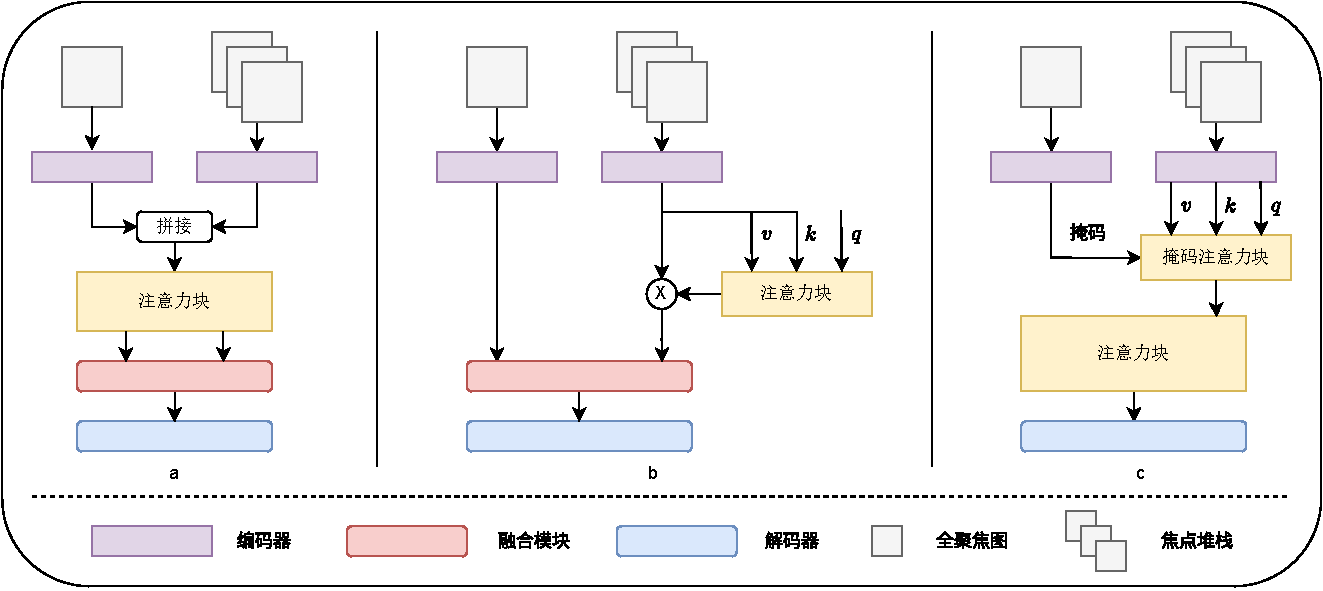
\includegraphics[width=0.95\linewidth]{figures/chapter4/task2_ins.drawio}
	\bicaption{光场模型范例}{TODO}  
	\label{cpt4_fig1:task2_ins}
\end{figure}
%
%
%
%
王等人~\cite{wang2023tenet}通过拼接焦点堆栈和全聚焦图特征,
一并送入Transformer编码器来,建立光场整体结构的感知模型。
如图~\ref{cpt4_fig1:task2_ins}~(a)~所示,
但是这种方式弱化了全聚焦图片特征和散焦图片特征之间的模态差异,两个模态之间的融合依然依赖后续的融合模块。
刘等人~\cite{liu2023lftransnet}只在焦点堆栈支路使用了Transformer结构。该方法聚合多尺度的焦点堆栈特征构造注意力矩阵,用一个可学习的权重来作为查询矩阵。通过注意力运算来汇总不同切片对显著性检测的贡献。如图~\ref{cpt4_fig1:task2_ins}~(b)~所示。
%
%
这种方法没有充分考虑两个模态之间的差异,仅在单焦点堆栈模态起到特征强化效果,只能考虑有限的特征表达。
% 
% 
% 
% 
\par
针对上述问题,本章提出一种基于视角增强的光场显著性目标检测方法。
此方法致力于从焦点堆栈和全聚焦图的协同感知入手,结合Transformer强大的注意力机制,提出了视角增强的注意力方法。
我们在一个简单的骨干网络之上,添加了视角增强编码器,
将全聚焦图的特征注入到焦点堆栈特征来增强每一张焦点堆栈图像的视角表达。
通过使用掩码注意力,注意力被限制在以全聚焦预测片段为中心的显著性特征上。
与标准的Transformer解码器中使用的交叉注意力(关注图像中的所有位置)相比,
被屏蔽的注意力能够达到更快的收敛效果和性能提高。
其次,为了进一并提高网络的表达能力,探索了使用基于跨图片像素的对比学习策略,
来引导网络学习统一的显著性语义和背景语义信息。
\par
% 
% 
% 
% 
为验证本方法的有效性,本章在 DUTLF, LFSD 以及 HFUT-LFSD 数据集上进行了实验,
同样获得了超越其他光场显著性分割网络的性能,为光场数据的应用奠定了基础。
% 
% 
% 为了进一步验证本方法的有效性,本章将提出的数据增强方法应用在当前最
% 好的光场显著性检测方法上,实验结果表明,本章的数据增强方法能够提升其它方法的
% 检测性能。
% 
% 
% 在视角增强编码器中,使用了掩码注意力,将
% ~
% 随着
% 然而,采集光场数据需要多组摄像头或相机矩阵,造成了高昂的成本。为了实现理想的光场显著性目标检测能力,除了设计合适的网络模型外,还需要大量高质量的光场数据。由于光场数据获取成本高,目前的方法通常采用数据增强手段来增加训练数据。传统的数据增强方法包括旋转、平移、裁剪和缩放等操作,但这些方式的变化有限,效果也不够显著。对于不同类型的光场数据,需要不同的增强方法,选择不当的方法可能会引入噪声,导致训练不稳定,降低模型性能。因此,如何稳定生成高质量的光场数据以实现数据增强的目标是当前需要解决的问题。
% 针对上述问题。  
% % task2_ins.drawio
% 
% 
% 
% 
\BiSection{方法介绍}{TODO}
% 
% 
本节将对本章提出的光场显著性目标检测网络模型进行详细介绍。
整体网络架构如图\textcolor{red}{TODO}所示。
本章采用了在显著性目标检测任务中经常被使用的PVT-v2作为骨干网络。
具体来说,给定一个尺寸为$W \times H$的RGB图像$I_{0}$和
焦点堆栈$\left \{  I_{1},I_{2},I_{3},\cdots,I_{12} \right \} $,
输入到编码器中以提取分辨率为$\frac{W}{2^{j}} \times \frac{H}{2^{j}} $
的特征$\left \{ F_{i}^{j},~j=1,2,3,4,5 \right \}$,
其中,$F_{i}^{j}$表示图像$I_{i}$在编码器第$j$层的特征,当$i=0$时,
$F_{i}^{j}$表示全聚焦图的特征,当$i=1,2,\cdots,12$时,$F_{i}^{j}$表示焦点堆栈图像的特征。
参考CPD的建议,低阶特征由于太简单而无法做出有效且可靠的预测,
本章只在高阶特征(即$F_{i}^{j},~j=2,3,4,5$)上执行解码操作。

\textcolor{red}{TODO}

本章工作提出的视角增强模块和跨图的像素对比学习策略将
分别在~\ref{chap:part4_view_enh}~以及~\ref{chap:part4_cons}~节进行详细介绍。


%
%
%
%
\BiSubsection{视角增强模块}{TODO}
\label{chap:part4_view_enh}
% 
% 
% 
% 
上下文特征已经被证明对图像分割很重要\textcolor{red}{TODO}.
然而,最近的研究表面,基于Transformer的模型收敛缓慢是由于交叉注意力层中的全局上下文,
因为交叉注意力需要许多训练周期才能学会关注局部对象区域。
假设局部特征足以更新查询特征,并且可以通过自注意力收集上下文信息,。
本节提出掩码注意力,可以看做是交叉注意力机制的一种变体,
仅关注每个查询的预测掩码的前景区域内。
\par
% 
% 
% 
% 
标准的交叉注意力(带残差路径)计算公式如下:
\begin{equation}
	X_{l}=softmax(Q_{l}K_{l}^{T})V_{l} + X_{l-1}
\end{equation}
其中,$l$是层索引,$X_{l} \in \mathbb{R}^{N\times C}$
是指$NC$在$l^{th}$层和
$ Q_{l} = f_{Q} \left ( X_{l-1} \right ) \in \mathbb{R}^{N \times C} $
的维度查询特征。$X_{0}$表示Transformer解码器的输入查询特征。
$K_{l},V_{l} \in \mathbb{R}^{H_{l}W_{l} \times C}$分别表示变换后的
输入图像特征$f_{K}(\cdot) $和$ f_{V}( \cdot )$,
$H_{l}$和$W_{l}$是图像特征的空间分辨率。
$f_{Q},~f_{K} $和$ f_{V} $是线性变换。
\par
% 
% 
% 
% 
掩码注意力通过以下方式调节注意力矩阵:
\begin{equation}
	X_{l}=softmax(M_{l-1} ~+~Q_{l}K_{l}^{T})V_{l} + X_{l-1}
\end{equation}
% 
% 
此外,在特征位置$(x,~y)$的掩码注意力掩码$M_{l-1}$是:
\begin{equation}
	M_{l-1}(x,~y)=\begin{cases}
		0  & \text{ if } M_{l-1}(x,~y)= 1\\
		-\infty & \text{ otherwise } 
	  \end{cases}
\end{equation}
% 
% 
在这里,$M_{l-1} \in \left \{  0,1\right \} ^{N \times H_{l}W_{l}} $是前一个
$l-1$层和
\textcolor{red}{TODO}
$M_{0}$是在将查询特征输入Transformer解码器之前,从全聚焦支路获得的二进制掩码预测。
\par
% 
% 
% 
% 
语义分割任务中,高分辨率的语义特征对提高模型性能具有显著帮助,特别是小物体的分割。
然而,使用越低级的语义信息,会带来更高的计算复杂度。
因此,引入了一种有效的多尺度策略,在控制计算量增加的同时,引入高分辨率特征。
首先,由最高层分辨率特征和下两层较低的分辨率特征组成特征金字塔,
并一次将多尺度的特征的一个分辨率特征传递给一个Transformer解码器层。
\par
% 
% 
% 
% 
具体来说,我们使用原始图像分辨率为$1/32,~1/16$和$1/8$的像素编码器产生的特征金字塔。
对于每一个分辨率,在输入到Transformer解码器之前他家正弦位置嵌入
$ e_{pos}\in \mathbb{R}^{H_{l}W_{l}\times C} $。
使用的Transformer解码器层,从最低分辨率到最高分辨率,如图所示。\textcolor{red}{TODO}。
网络总共重复这个3层的Transformer解码器$L$次。因此,网络最终的Transformer解码器层有$3L$层。
更具体的说,前三层介绍分辨率$H_{1}=H/32,H_{2}=H/16,H_{3}=H/8$
和$W_{1}=W/32,W_{2}=W/16,W_{3}=W/8$的特征图,其中$H$和$W$是原始图像分辨率。
之后的所有层都以循环的方式重复此模式。

\BiSubsection{感知对比学习策略}{TODO}
\label{chap:part4_cons}
% 
% 
% 
% 
对比学习常用于无监督中视觉表示学习。
无监督对比学习旨在学习CNN编码器$f_{CNN}$将每个训练图像转换为特征向量表示$v=f_{CNN}(I) \in \mathbb{R}^{D}$,
使得$v$能够描述图片$I$。
为了实现这一目标,
对比学习通过区分正样本(一个增强版本的图像$I$)
和多个负样本(从训练集中随机挑选的图像,但是不包括$I$)来进行训练。
在对比学习中,会集成使用InfoNCE损失函数,其公式如下:
\begin{equation}
	\mathcal{L} _{I}^{NCE}=-log \frac{exp(v \cdot v^{+ }/\tau )}
{exp(v \cdot v^{+}/\tau )+ \sum_{v^{-}\in N_{I}} exp(v \cdot v^{-}/\tau )} 
\end{equation}
其中$v^{+}$是正样本图像$I$的嵌入,$N_{I}$是包含负样本的嵌入,$\cdot$表示内(点)积,
$\tau >0$是温度超参数。损失函数在计算前,还需要对所有嵌入进行$\ell_{2}$归一化。
\par
% 
% 
% 
% 
另一个需要解释的概念是知识库。
一些最近的研究表明,大量的负样本(即$N_{I}$)在无监督对比学习中至关重要
\cite{wu2018unsupervised,chen2020improved,he2020momentum}。
但是负样本的数量受到小批量(mini-batch)大小的限制,
最近的对比学习方法利用大型外部存储器来储存更多的负样本。
具体来说,一些方法\cite{wu2018unsupervised}直接将所有训练样本的嵌入表示存储在内存中,
但是很容易受到异步更新的影响。
其他一些人选择用一个队列保存最后几个批次的的嵌入\cite{wang2020cross,chen2020improved,he2020momentum}。
在\cite{chen2020improved,he2020momentum}中,
存储的嵌入表示还可以通过编码器网络$f_{CNN}$的动量更新而进行动态更新。
\par
% 
% 
% 
% 
像素级交叉熵损失。
在显著性分割的背景下,图像$I$的每个像素$i$需要被分类为显著性的前景类或者背景类。
当前的方法通常将此任务视为逐像素分类问题。具体来说,
令$f_{FCN}$作为FCN编码器(例如ResNet\cite{he2016deep}),它为图像$I$生成密集特征预测
$I\in \mathbb{R}^{ H \times W \times D}$,
从中可以导出每个像素的嵌入$i \in  \mathbb{R}^{D}$。
之后分割头$f_{SEG}$把图像$I$映射到分类激活图
$Y=f_{SEG}(I) \in \mathbb{R}^{H\times H \times |C|}$。
进一步设$y=\left [ y_{1},\dots, y_{C} \right ] \in\mathbb{R}^{C}$
是像素$i$的非归一化得分向量(称为logit),可以从$Y$导出,
即$y \in Y$。
给定像素$i$的真实标签$\bar{c} \in C$,交叉熵使用softmax进行优化:
\begin{equation}
	\mathcal{L}_{i}^{CE}=-1_{\bar{c}}^{\top } log(softmax(y))
	\label{chpt4:eq:loss_softmax}
\end{equation}
% 
% 
% 
% 
其中,$1_{\bar{c}}$表示$\bar{c}$的one-hot编码,
其中的对数算法是逐元素计算的:
\begin{equation}
softmax(y_{c}) = \frac
{exp(y_{c})}
{ 
\sum_{{c}'=1 }^{|C|} 
exp(y_{{c}'}) 
} 
\end{equation}
% 
% 
% 
% 
这种独立训练目标的设计有两个主要限制。
1)它独立的乘法像素级预测,但忽略像素之间的关系~\cite{zhao2019region}。
2)由于使用了softmax,损失仅取决于logits之间的相对关系,
不能直接得到监督学习的表示~\cite{pang2019rethinking}。
这两个问题很少被注意到;只有少数结构感知损失被设计来解决1),
通过考虑像素亲和力~\cite{ke2018adaptive},
优化交叉测量~\cite{berman2018lovasz},
或者最大化真值和预测图之间的互信息~\cite{zhao2019region}。然而,
这些替代损失仅考虑图像内像素之间的依赖性(即全局上下文),
而不考虑图像不同像素之间的语义相关性(即全局结构)
\par
% 
% 
% 
% 
在这项工作中,我们构造了一种逐像素对比学习的方法,通过规范嵌入空间并探索训练数据的全局结构来解决
问题1)和问题2)。
我们首先扩展了公式。去适配我们有监督的密集图像预测任务。
总的来说,我们的对比损失函数计算的是数据样本中每张图像的像素。
此外,对于具有真实语义标签的像素$i$,正样本也属于类的其他像素,
而负样本是属于其他类的像素。
我们的有监督形式的逐像素对比损失定义为:
\begin{equation}
\mathcal{L} _{I}^{NCE}= 
\frac{1}{|P_{i}|}
\sum_{i^{+}\in P_{i}}^{}  
-log \frac
{exp(i \cdot i^{+ }/\tau )}
{exp(i \cdot i^{+}/\tau )+ \sum_{i^{-}\in N_{I}} exp(i \cdot i^{-}/\tau )} 
\label{chpt4:eq:con_loss}
\end{equation}
% 
% 
% 
% 
其中$P_{i}$和$N_{i}$分别表示像素$i$的正样本和负样本的像素嵌入集合。
并且,正负样本和锚点$i$不局限于统一图像。如公式~\ref{chpt4:eq:con_loss}~所示,
这种基于像素到像素对比度的损失设计的目的是通过
将同一类像素样本拉进
并
将不同类样本推开来学习其隐含的嵌入表示。
\par
% 
% 
% 
% 
公式~\ref{chpt4:eq:loss_softmax}~中的像素交叉熵损失以及
在公式~\ref{chpt4:eq:con_loss}~中的对比损失是互补的。
前者能让显著性分割网络学习对前背景分类有意义的判别性像素特征,
而后者通过显示探索像素样本之间的全局语义关系,
有助于规范嵌入空间,
提高类内紧凑性和类间可分离性。
因此总体训练目标是:
\begin{equation}
	\mathcal{L}^{SEG}=\sum_{i}\left ( 
		\mathcal{L}_{i}^{CE} + 
		\lambda \mathcal{L}_{i}^{NCE}  
	\right ) 
\end{equation}
% 
% 
% 
% 
其中$\lambda > 0 $是系数,$\mathcal{L}^{SEG}$
学习到的像素嵌入变得更加紧凑且分离良好。
这表明,通过利用一元交叉熵损失和成对比度量损失的优势,
显著性分割网络可以生成更具辨别力的特征,
从而产生更有希望的结果。

稍后在\todo 和\todo 中提供了定量分析。


像素与区域的对比。
如\todo 所述,记忆是一项关键技术,
有助于对比学习利用海量数据来学习良好的表示。
然而,由于我们的密集预测设置中有大量的像素样本,
并且其中大多数是冗余的(即从相似对象区域采样),
因此像传统存储器一样直接存储所有训练像素样本\todo ,
会大大减慢学习过程。
\par
% 
% 
% 
% 
在队列中维护最后几个批次,例如\todo,
也不是一个最优的选择,
因为最近的批次仅包含有限数量的图像,
降低了像素样本的多样性。
因此,我们选择分别为前景类和背景类维护一个像素队列。
对于每个类别,仅从最新小批量中的每个图像中随机选择少量像素$V$,
并将其拉如队列,大小为$T \gg  V$。
% 
% 
% 
% 
在实践中,我们发现这种策略非常高效并且有效,但是欠采样像素嵌入
太稀疏,无法完全捕获图像内容。
因此,我们进一步构建了一个区域存储库,用于存储从图像片段(即语义区域)
吸收的更具代表性的嵌入。


具体来说,对于总共有$N$个训练图像和$|C|=2$个分割类,
我们的区域内存的大小为$|C|\times N \times D$,
其中$D$是像素嵌入的维度。区域内存中的第$(\bar{c},~n)$
个元素是通过平均池化第n个图像中标记为$c$类别的像素的所有嵌入而获得的
$D$维特征向量。
使用区域内存有两个优点:

1)以较低的内存消耗存储更具代表性的像素样本;
2)允许我们的像素对比损失~\ref{chpt4:eq:con_loss}~进一步探索像素与区域的关系。
关于2),当计算属于$\bar{c}$类别的锚像素$i$时,计算公式~\ref{chpt4:eq:con_loss}~时,
具有相同类别$\bar{c}$的存储区域嵌入被视为正例,
而具有其他类别$C/ \bar{c}$ 的区域嵌入被视为负例。
% 
% 
% 
% 
\par
对于像素存储器,大小为$|C|\times T \times D$。
因此,对于整个内存(记为 $M$ )来说,总大小为$|C| \times (N+T) \times D$。
在\todo 中检查了$M$ 中的像素嵌入和区域嵌入。









% 
% 
% 
% 
\BiSubsection{训练过程}{TODO}


%\\
%\\
%\\
%\\
\BiSection{实验结果与分析}{TODO}

\BiSubsection{实验设置}{TODO}

\BiSubsection{消融实验}{TODO}

\BiSubsection{对比实验}{TODO}


%\\
%\\
%\\
%\\
\BiSection{本章总结}{TODO}